%! TeX program = lualatex
%---------------------------ALLGEMEINE IMPORTS-------------------------------------
\documentclass[12pt,english,ngerman]{scrartcl}

\input{./protokoll_template/template.latex/input/shared_preamble.tex}

    % Kopfzeile
\ihead{WS22\\11.11.2022}
\chead{\textsc{Stark} Matthias - 12004907 \\ \textsc{Philipp} Maximilian - 11839611}
\ohead{FLAB 1 \\ Zählrohr}
    % Fußzeile

\begin{document}
%\includepdf{}
\tableofcontents
\newpage

\section{Aufgabenstellung\label{Auf}}



\begin{itemize}
    \item Messung der $\alpha$, $\beta$ und $\gamma$ Strahlung ohne und mit verschiedenen dicken Abschirmungen
    \item Aufnahme der Zählrohrcharakteristik
    \item Aufnahme der Zählstatistik
    \item Bestätigung des Abstandsgesetzes
    \item Bestimmung der Endpunktsenergie über Absorption in Aluminium
    \item Aufnahme des Energiespektrums von $\beta$ Strahlung mit Magnetspektrometer
    \item Aufnahme und Kalibrierung des $\gamma$ Spektrums
    \item Aufnahme des komplexen $\gamma$ Spektrums und seinen Zerfallsprodukten
\end{itemize}

\section{Grundlagen}\label{Grund}

\subsection{Radioaktivität}
Nicht alle, in der Natur vorkommenden, Isotope sind stabil und zerfallen so mit einer gewissen Halbwertszeit $\tau$.
Bei diesen Zerfällen kann grundsätzlich zwischen verschiedenen Zerfällen unterschieden werden.

Bei $\alpha$ - Zerfall wird ein Heliumkern ausgestoßen, was sich schließlich auf die Massen und Ordnungszahl auswirkt.

Bei $\beta$ - Zerfall muss zwischen $\beta^+$ und $\beta^-$ unterschieden werden.
$\beta^-$ - Zerfall wird durch die Umwandlung eines Neutrons in ein Proton hervorgerufen, wodurch ein Elektron und ein 
Elektron-Antineutrino ausgestoßen werden, um die Erhaltungssätze nicht zu verletzen.
$\beta^+$ - Zerfall kommt in der Natur seltener vor, funktioniert aber nach dem gleichen Prinzip, mit dem Unterschied, 
dass hier die Ordnungszahl erhöht wird.

Bei $\gamma$ - Zerfall werden keine Teilchen sondern hochfrequente Wellen abgestrahlt. Diese kommen zustande,
wenn das Isotop nach $\alpha$ oder $\beta$ - Zerfall noch in einem angeregten Zustand ist, wodurch durch die
$\gamma$ - Strahlung Spektren entstehen, die signifikant für bestimmte Elemente sind, was im Laufe des Versuchs 
genutzt wird.


Weil diese Zerfälle immer nach einem bestimmen Schema ablaufen, können sogenannte Zerfallsreihen angeschrieben werden, 
wie beispielsweise die Zerfallsreihe von \ch{^{226}_{88}Ra} in \autoref{fig:zerfallsreihe}. Daraus kann abgelesen
werden, welche Zerfälle vorliegen und auch welche Halbwertszeiten diese haben, wie häufig die Zerfälle also auftreten.

\begin{figure}[H]
  \begin{center}
  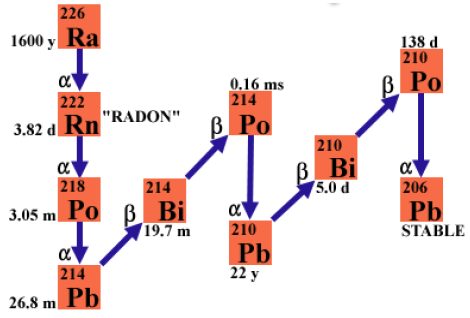
\includegraphics[width=0.5\textwidth]{./figures/zerfallsreihe.png}
	\end{center}
	\caption{Zerfallsreihe \ch{^{226}_{88}Ra} \cite[]{}}
	\label{fig:zerfallsreihe}
    
\end{figure}


Die Intensität $I$ radioaktiver Strahlung folgt dabei dem Abstandsgesetz, welches folgendermaßen definiert werden kann:
\begin{equation}
  I \propto \frac{1}{l^2}
\end{equation}

$l$ entspricht dabei dem Abstand zur radioaktivenn Quelle.

Für die Absorption von radioaktiver Strahlung gilt das Beer-Lambertsche Absorptionsgesetz:
\begin{equation}
  I = I_0 \exp(-\mu d)
\end{equation}

$I$ beschreibt dabei die Intensität der Strahlung nach der Barriere, $I_0$ die Anfangsintensität, 
$\mu$ den Absorptionskoeffizienten der Barriere und $d$ die Dicke der Barriere.

Aus den Absorptionskoeffizienten kann die Ruheenergie $E_0$ nach folgender Formel berechnet werden:
\begin{equation}
  \frac{\mu}{\rho} = 17.6 E_0^{-1.39}
\end{equation}

$\rho$ beschreibt dabei die Dichte der Barriere, dessen Absorptionskoeffizient bestimmt wurde.\cite[]{}


\subsection{Zählrohr}

Im Versuch wird ein sogenanntes Geiger-Müller-Zählrohr verwendet, dessen schematischer Aufbau in \autoref{fig:zahlrohr} ersichtlich ist.
Es besteht im wesentlichen aus einem mit Zählgas gefüllten Metallrohr, durch dessen Mitte ein dünner Draht, der als Anode fungiert,
läuft. Auf diesen Draht wird eine Spannung angelegt. Trifft nun ein zu detektierendes Teilchen auf das Fenster des 
Zählrohrs, können Atome im Zählgas angeregt werden, welches durch die angelegte Spannung zur Anode hin beschleunigt 
wird. Durch Stöße im Gas wird ein Lawineneffekt ausgelöst, der schlussendlich als Peak von der Anode verzeichnet werden kann.

\begin{figure}[H]
  \begin{center}
  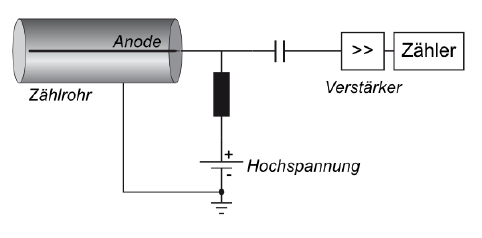
\includegraphics[width=0.5\textwidth]{./figures/zahlrohr.png}
	\end{center}
	\caption{schematischer Aufbau des Zählrohrs \cite[]{}}
	\label{fig:zahlrohr}
    
\end{figure}

Der charakteristische Verlauf der Kurve des Zählrohrs ist in \autoref{fig:zchar} ersichtlich.
Dabei sind die einzelnen Bereiche zu unterscheiden \cite[]{} :

%todo Liste vlt in Aufzählung mit röm nummern ändern
\begin{itemize}
  \item Hier werden die Elektronen aufgrund der angelegten Spannung zur Anode hin Beschleunigt.
  \item In diesem Bereich ist eine Sättigung erreicht. Es bewegen sich also nicht alle Atome direkt zur Anode.
  \item Hier ist die Spannung so hoch, dass die Atome auf den Weg zur Anode mit anderen Atomen zusammenstoßen, wodurch der Lawineneffekt ausgelöst wird.
  \item In diesem Bereich befindet sich das sogenannte Geiger-Müller-Plateau. Hier ist der Betrieb quasi nicht spannungsabhängig, weshalb dies auch der gewünschte Messbereich ist.
  \item Eine weitere Erhöhung in diesen Bereich erhöht zwar auch die Zählrate, zerstört aber auf Dauer den Zähler, weshalb dieser Bereich zu meiden ist.
\end{itemize}

\begin{figure}[H]
  \begin{center}
  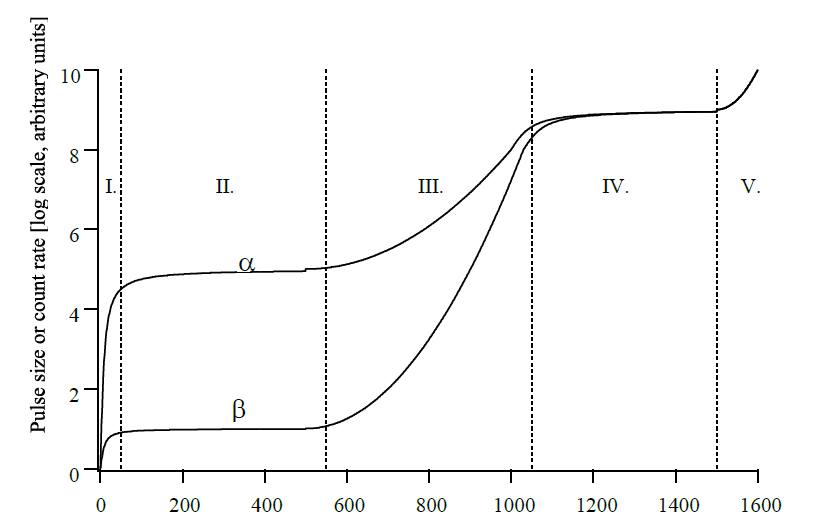
\includegraphics[width=0.8\textwidth]{./figures/zcharakteristik.png}
	\end{center}
	\caption{charakteristische Kurve des Zählrohrs für verschiedene Arten von Strahlung für die 
  Bereits erklärten Spannungsbereiche \cite[]{}}
	\label{fig:zchar}
    
\end{figure}



\subsection{Magnetspektrometer}

Die Funktionsweise eines Magnetfeldspektrometer basiert auf der Lorentzkraft. So wird $\beta$ - Strahlung, die im Grunde aus 
Elektronen besteht, in einer Kreisbahn abgelenkt und so von der $\gamma$ - Strahlung getrennt. Der schematische Aufbau eines
Magnetfeldspektrometers ist in \autoref{fig:magnetspektrometer} ersichtlich. In der Abbildung ist klar die Kreisförmige
'Flugbahn' der $\beta$ - Strahlung vom Präparat zum Zählrohr sichtbar.\cite[]{}


\begin{figure}[H]
  \begin{center}
  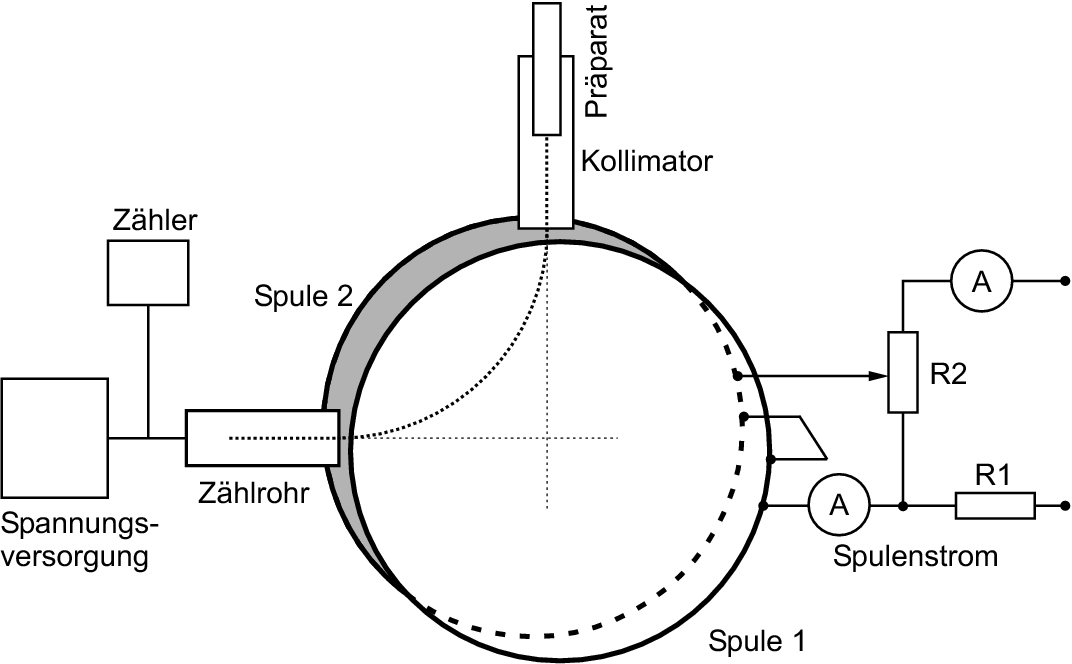
\includegraphics[width=0.8\textwidth]{./figures/fig5.png}
	\end{center}
	\caption{schematischer Aufbau des Magnetfeldspektrometers \cite[]{}}
	\label{fig:magnetspektrometer}
    
\end{figure}


\subsection{Szintilationszähler}

Der schematische Aufbau eines Szintilationszählers ist ist in \autoref{fig:szintilationszahler} sichtbar.
Grundsätzlich besteht er aus einem Szintilartor, bei dem durch die Anregung der Strahlen Photonen ausgesendet werden, 
die von der Photokathode erfasst werden. Dahinter befindet sich ein Photomultiplier, an dessen Ende schlussendlich
die vielen Elektronen von der Anode abgegriffen werden, was das erhaltene Signal darstellt.\cite[]{}

\begin{figure}[H]
  \begin{center}
  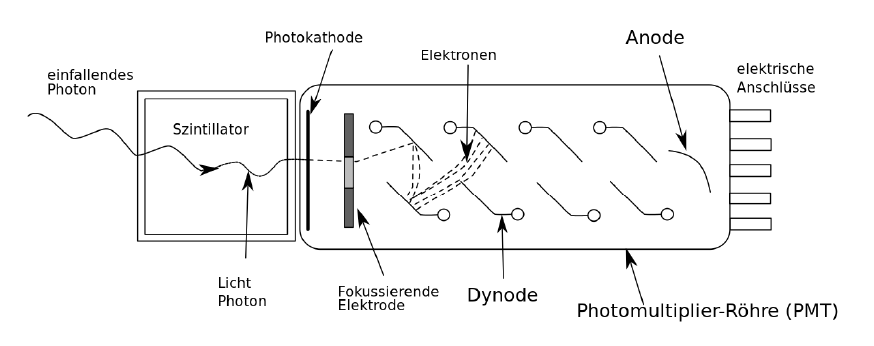
\includegraphics[width=0.8\textwidth]{./figures/szintilationszahler.png}
	\end{center}
	\caption{schematischer Aufbau und Strahlengang im Szintilationszähler \cite[]{}}
	\label{fig:szintilationszahler}
    
\end{figure}


\section{Versuchsanordnung}\label{sec:Versuchsanordnung}

Im Laufe des Versuchs wurden 3 verschiedene Aufbauten verwendet die im Verlauf modifiziert wurden.

\subsection{Digitalzähler}\label{aufbau_Digz}

Für den ersten Teil des Versuchs wird folgender Versuchsaufbau aus
\autoref{fig:digz} realisiert. Dabei wird das Präparat in die dafür vorgesehene
Halterung geschoben, hinter der sich das Zählrohr befindet, welches mit dem
Digitalzähler verbunden ist, wodurch ein einfaches Ablesen der Counts
ermöglicht wird. Auf der optischen Bank kann der Abstand zwischen Präparat und
Zählrohr variiert und abgelesen werden. Dabei ist zu beachten, dass die
abgelesene Distanz auf der optischen Bank nicht dem tatsächlichen Abstand
zwischen Probe und Zählrohr entspricht, da sich diese nicht direkt über den
Sockel befinden. Um im späteren Verlauf des Versuchs die Aluminiumbleche zu
befestigen, wird die entsprechende Halterung auf die optische Bank gesteckt.

\begin{figure}[H]
  \begin{center}
  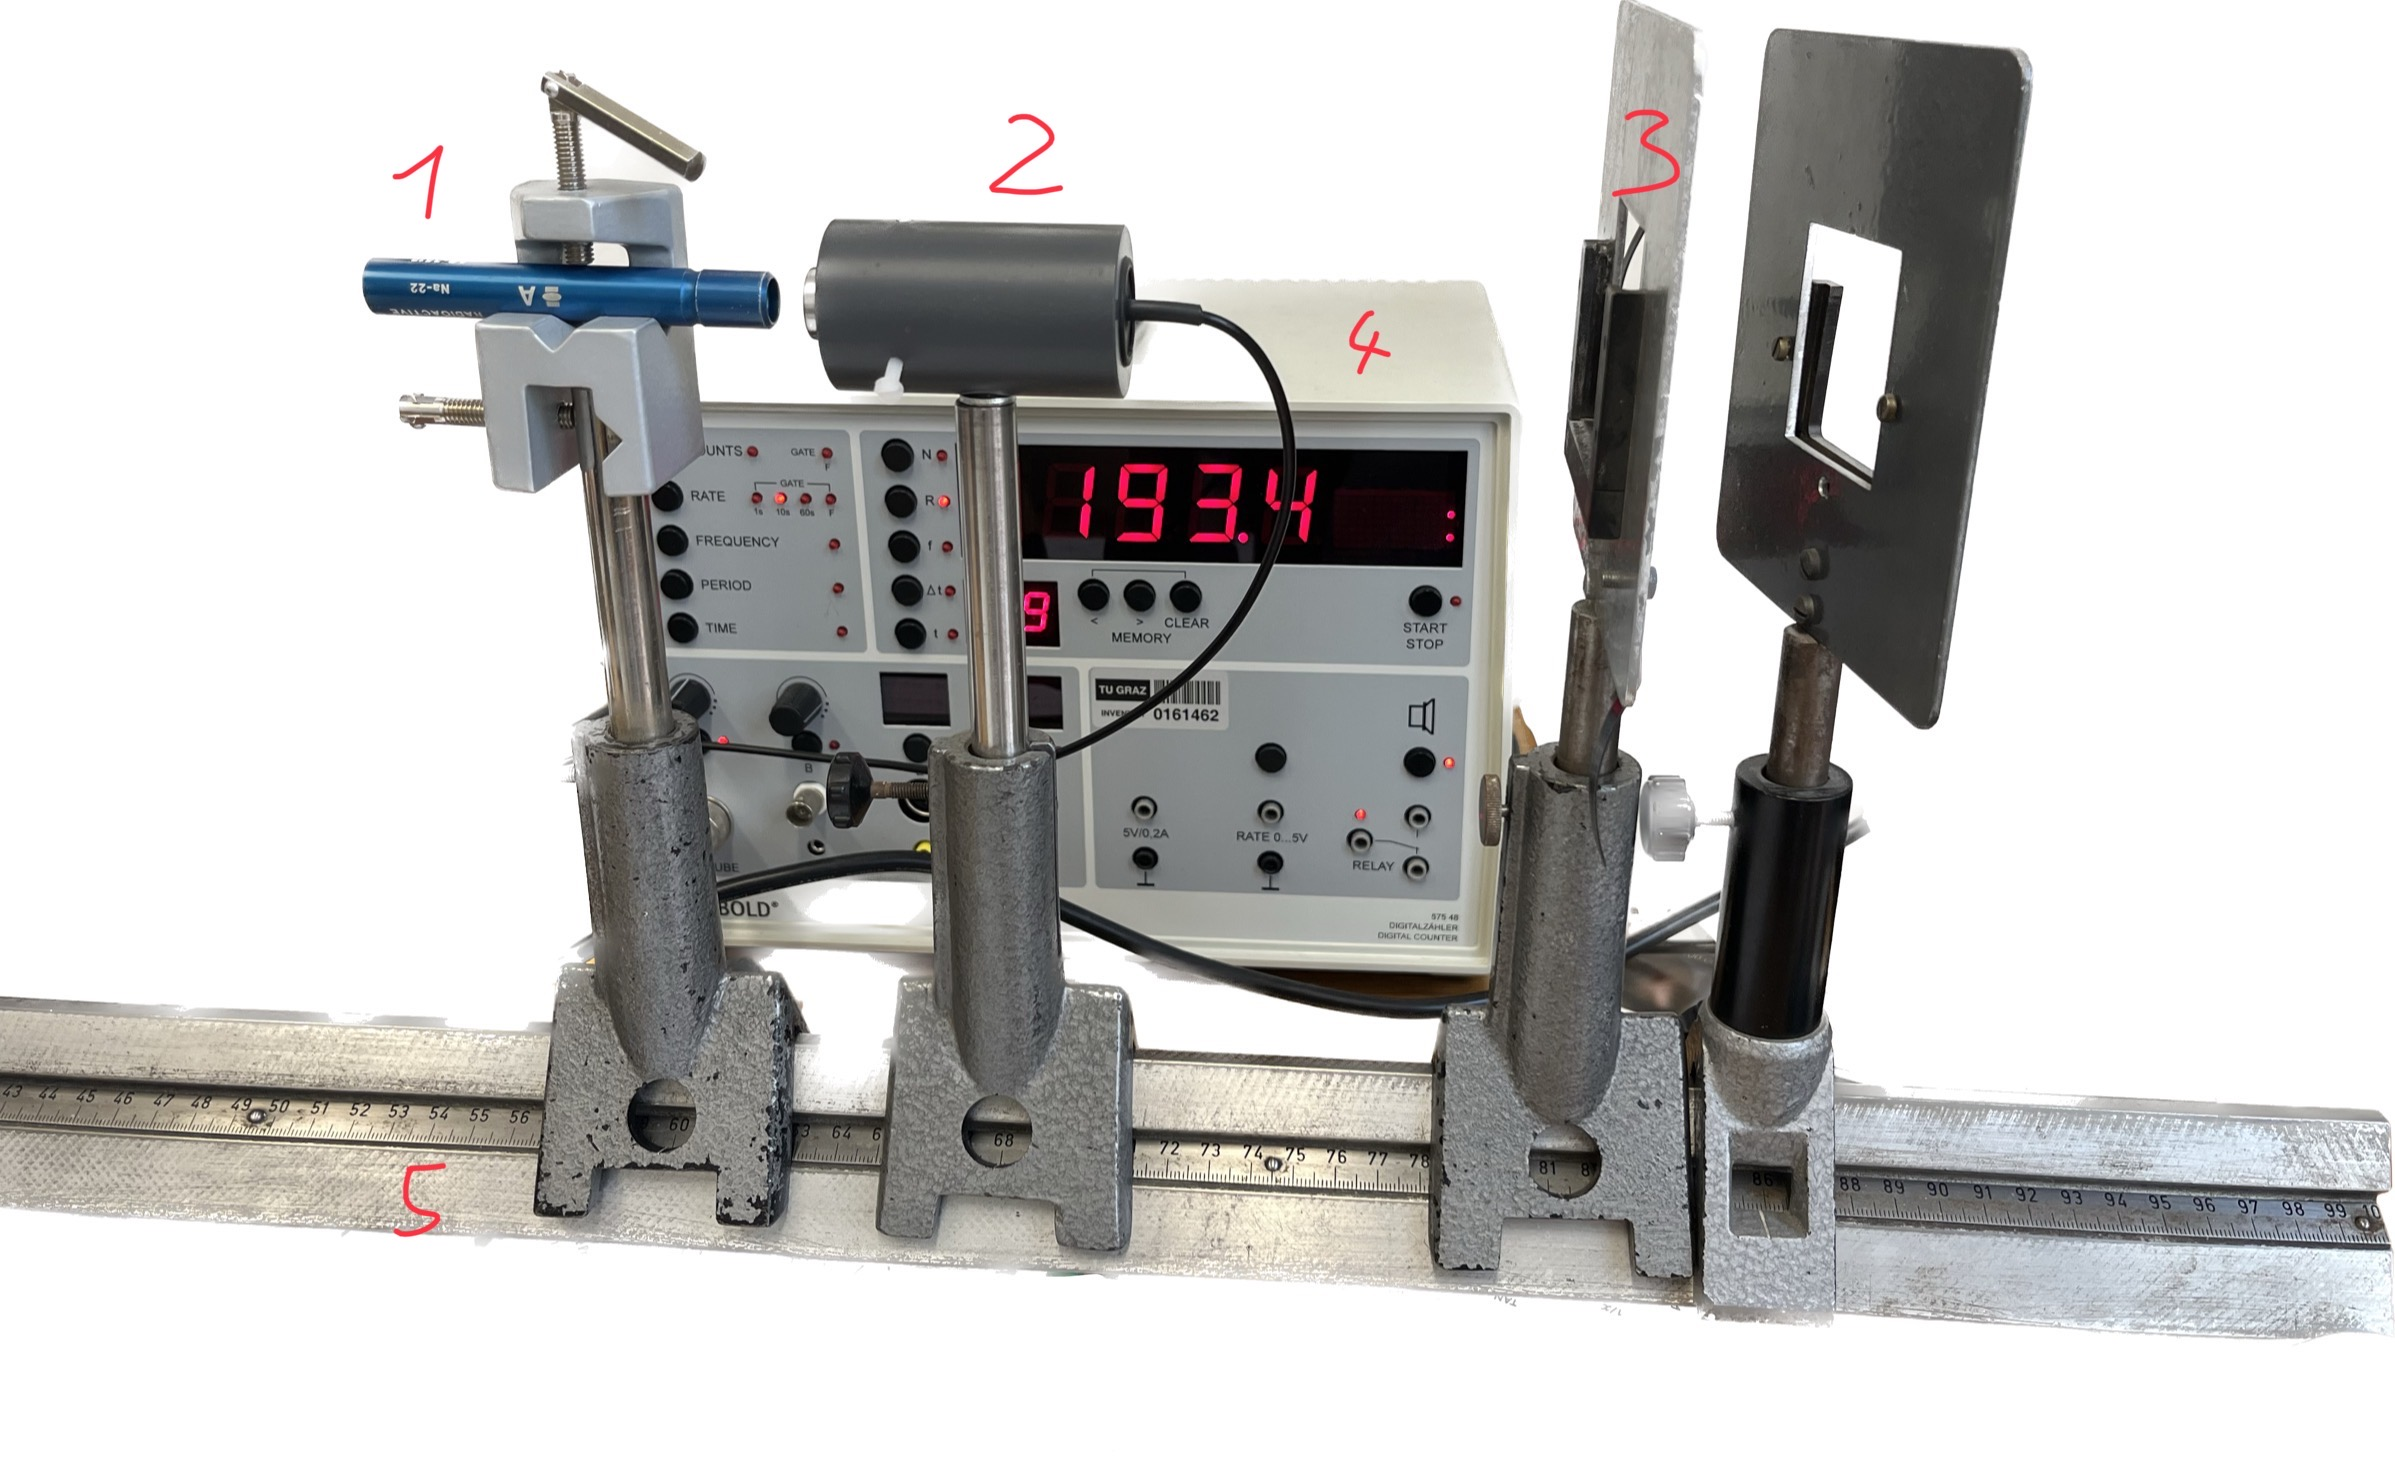
\includegraphics[width=0.8\textwidth]{./figures/digz.png}
	\end{center}
	\caption[Aufbau des Digitalzähler]{Aufbau des Digitalzähler \\ 
    1 $\dots$ Halterung für radioaktive Quelle \\ 
    2 $\dots$ Zählrohr \\
    3 $\dots$ Halterung um später das Aluminium zu Befestigen \\ 
    4 $\dots$ Digitalzähler \\ 
    5 $\dots$ optische Bank um den Abstand zu variieren}
	\label{fig:digz}
    
\end{figure}

\subsection{Magnetfeldspektrometer}\label{sec:aufbau_Magnetfeldspektrometer}

Um $\beta$ Strahlung messbar zu machen, wird folgender Aufbau aus
\autoref{fig:mag} verwendet. Dabei wird das radioaktive Präparat in das dafür
vorgesehene Loch gesteckt. Durch die Spule wird ein Magnetfelds erzeugt,
wodurch die Betastrahlung aufgrund von Lorentzkraft abgelenkt wird, weshalb die
Hallsonde auch schräg zur Quelle angeordnet ist. Dies stellt sicher, dass keine
Gammastrahlung gemessen wird. Die Stärke des Magnetfelds wird durch das
Netzgerät bestimmt.


\begin{figure}[H]
    \begin{center}
    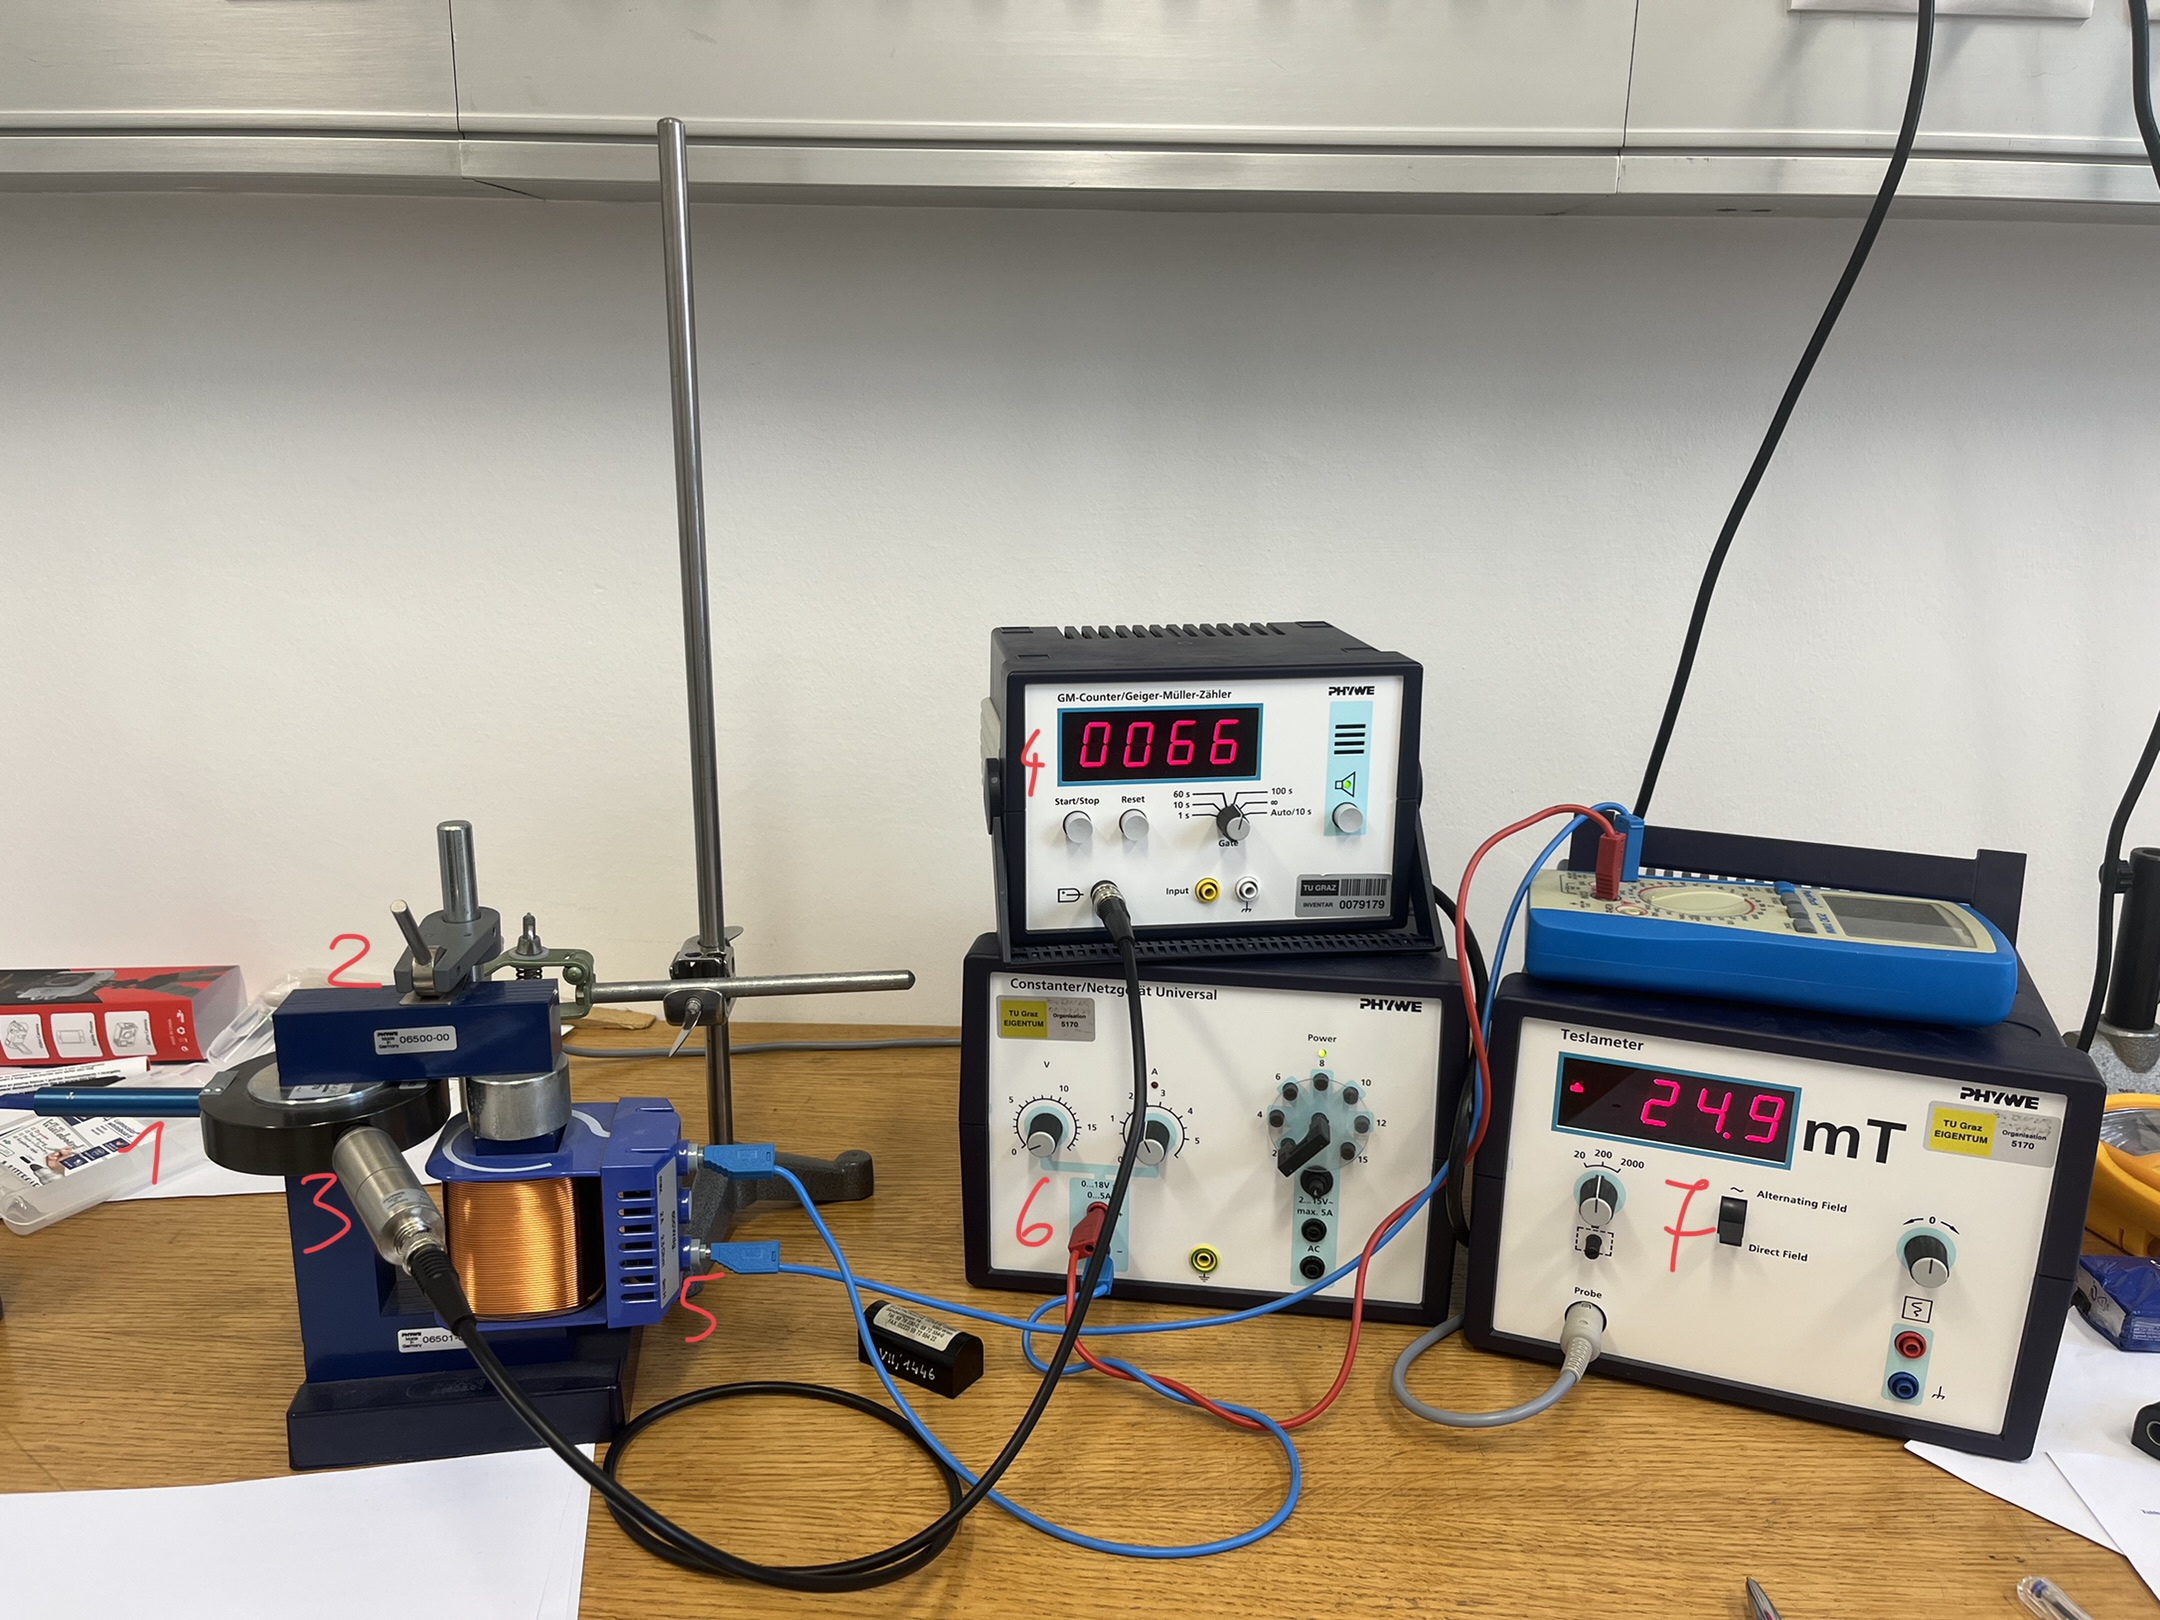
\includegraphics[width=0.8\textwidth]{./figures/mag_new.png}
      \end{center}
      \caption[Aufbau des Magnetfeldspektrometers]{Aufbau des Magnetfeldspektrometers \\ 
        1 $\dots$ Radioaktive Quelle \\
        2 $\dots$ Hallsonde (nicht sichtbar im Foto) \\
        3 $\dots$ Epfänger des Geiger-Müller-Zählers \\
        4 $\dots$ Anzeige des Geiger-Müller-Zählers \\
        5 $\dots$ Spule um das Magnetfeld zu erzeugen \\
        6 $\dots$ Netzgerät für das Magnetfeld (Stecker um die Polung des Magnetfelds zu Ändern) \\
        7 $\dots$ Teslameter um die Stärke des Magnetfelds zu bestimmen}
      \label{fig:mag}
      
  \end{figure}


\subsection{Szintilationszähler}\label{aufbau_szinti}

Der Aufbau des Szintilationszählers ist in folgender \autoref{fig:szinti}
sichtbar. Die radioaktive Quelle wird in die, dafür vorgesehene, Halterung ober
den Szintilationszähler gesteckt. Um eine Auswertung am PC zu ermöglichen, wird
ein Cassy-Lab als Schnittstelle verwendet.

\begin{figure}[H]
    \begin{center}
    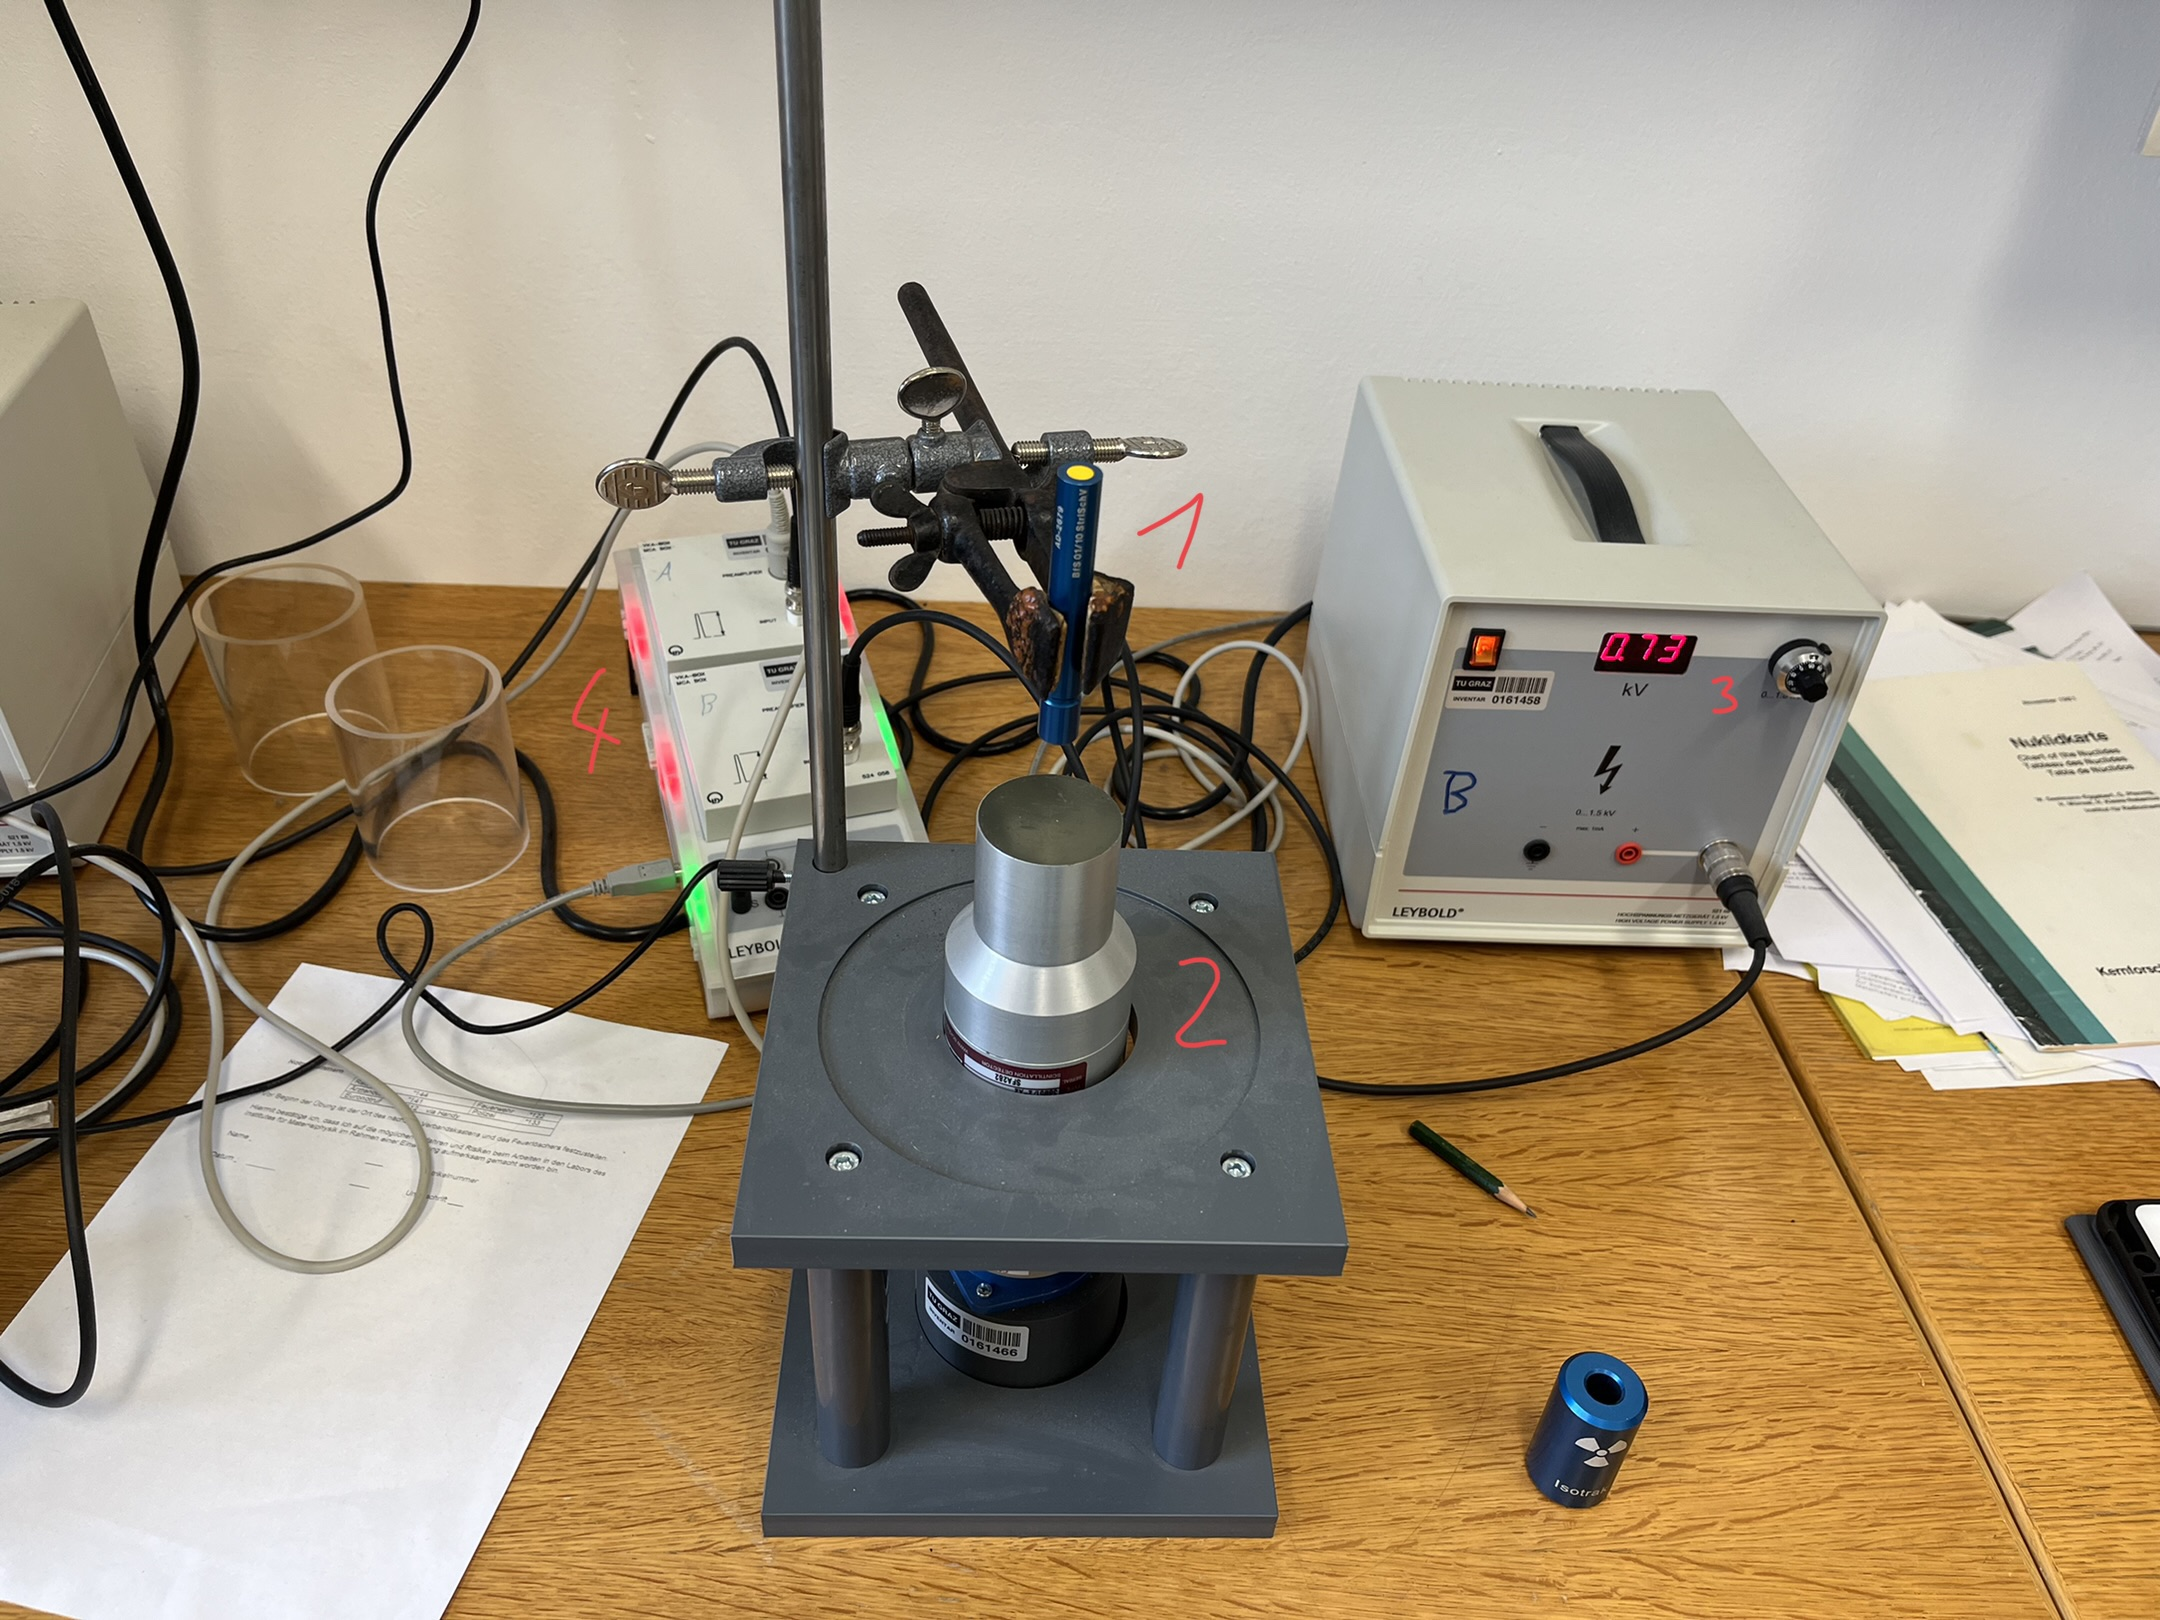
\includegraphics[width=0.8\textwidth]{./figures/szinti.png}
      \end{center}
      \caption[Aufbau des Szintilationszählers]{Aufbau des Szintilationszählers \\ 
        1 $\dots$ Radioaktive Quelle \\ 
        2 $\dots$ Szintilationszähler \\
        3 $\dots$ Spannungsgenerator \\ 
        4 $\dots$ Cassy-Lab um Auswertung am PC zu ermöglichen}
      \label{fig:szinti}
      
  \end{figure}


\section{Geräteliste}

Die Geräteliste wurde uns freundlicherweise zur Verfügung gestellt und nur um die verwendeten Strahlungsquellen ergänzt. \cite[]{}

\begin{table}[H]
  \caption{verwendete Geräte}
  \begin{tabular}{|l|l|l|l|}
    \hline
    Gerätetyp              & Hersteller & Typ             & Inventar-Nr \\ \hline
    Digitalzähler          & Leybold    & 57548           & 161462      \\ \hline
    Geiger-Müller-Zählrohr & Leybold    & 5240331         &             \\ \hline
    $\beta$ Spektrometer   & Phywe      &                 &             \\ \hline
    Netzgerät Universal    & Phywe      & Set Betaspektr. &             \\ \hline
    Geiger-Müller Zähler   & Phywe      & P2523200        & 79179       \\ \hline
    Spule mit Eisenkern    & Phywe      &                 &             \\ \hline
    Teslameter             & Phywe      &                 &             \\ \hline
    Hochspannungsnetzgerät & Leybold    & 52188           & 161458      \\ \hline
    Szintilationszähler    & Leybold    & 559901          & 161460      \\ \hline
    Sensor-Cassy 2         & Leybold    &                 & 161474      \\ \hline
    VKA Box                & Leybold    & 524058          & 161465      \\ \hline
    \ch{^{22}_{11}Na}      &            &                 & AG-3518     \\ \hline
    \ch{^{90}_{38}Sr}      &            &                 & AG-3676     \\ \hline
    \ch{^{226}_{88}Ra}     &            &                 & 559435      \\ \hline
    \end{tabular}
\end{table}

\section{Versuchsdurchführung \& Messergebnisse}\label{sec:Durchfuhrung}

\subsection{Messung der \texorpdfstring{$\alpha$}{alpha}, \texorpdfstring{$\beta$}{beta} und 
\texorpdfstring{$\gamma$}{gamma} Strahlung ohne und mit verschiedenen dicken Abschirmungen}

Um die Abschirmung Strahlungen zu Messen, wir der Versuchsaufbau, wie in
\autoref{aufbau_Digz} beschrieben, vorgenommen. Die Torzeit am Digitalzähler
wird dabei auf \SI{10}{\second} gestellt. Als radioaktive Quelle wird
\ch{^{22}_{11}Na} verwendet, welche, wie bereits beim Aufbau erklärt, in die
dafür vorgesehene Halterung gesteckt wird. Der Abstand zwischen der Quelle und
dem Zählrohr wird dabei so gering gewählt, dass die dickste Abschirmungsprobe
problemlos dazwischen gehalten werden kann, ohne gegen die Probe oder das
Zählrohr zu stoßen. Diese Distanz zwischen der radioaktiven Quelle und dem
Zählrohr wird mit einem Lineal vermessen und beträgt \SI{15(2)}{\mm}. Die
unterschiedlichen Abschirmungen werden der Reihe nach in den Aufbau gehalten
und die entsprechenden Zählraten notiert, was in folgender
\autoref{tab:abschirmung} sichtbar ist. Dabei ist zu Beachten, dass die
jeweilige Abschirmung die gesamte Torzeit im Aufbau ist und man damit nicht
gegen die Probe oder das Zählrohr stößt.

%tab einfügen (von zettel)
\begin{table}[H]
  \caption[Erhaltene Zählraten bei verschiedenen Abschirmungsmaterialien]{Erhaltene Zählraten bei 
  verschiedenen Abschirmungsmaterialien bei einer Torzeit von \SI{10}{\second} und einem 
  Abstand der radioaktiven Quelle von \SI{15(2)}{\mm}. Die Unsicherheit beträgt dabei für alle Zählraten \SI{}{} \\ 
  $ z_{Luft} \dots$ erhaltene Zählrate ohne Abschirmung \\
  $ z_{\mathrm{Papier}} \dots$ erhaltene Zählrate mit einem Blatt Papier als Abschirmung \\
  $ z_{\mathrm{Lineal}} \dots$ erhaltene Zählrate mit einem Lineal als Abschirmung (Dicke = \SI{2.1(0.05)}{\mm})\\
  $ z_{\mathrm{Kunststoff}} \dots$ erhaltene Zählrate mit einer CD und zugehörigen Soulcase als Abschirmung \\
  $ z_{\mathrm{Alu \num{0.4}}} \dots$ erhaltene Zählrate mit mit einem Aluminiumblech als Abschirmung, Dicke = \SI{0.4(0.05)}{\mm}\\
  $ z_{\mathrm{Alu \num{0.8}}} \dots$ erhaltene Zählrate mit mit einem Aluminiumblech als Abschirmung, Dicke = \SI{0.8(0.05)}{\mm}\\
  $ z_{\mathrm{Alu \num{4}}} \dots$ erhaltene Zählrate mit mit einem Aluminiumblech als Abschirmung, Dicke = \SI{4(0.05)}{\mm}\\}
  \label{tab:abschirmung}
  \begin{center}
    \begin{tblr}{colspec={S[table-format=3.1(1)]|S[table-format=3.1(1)]|S[table-format=1.1(1)]|S[table-format=2.1(1)]|S[table-format=2.1(1)]|S[table-format=1.1(1)]}}
{{{$z_{\mathrm{Luft}}$}}} & {{{$z_{\mathrm{Papier}}$}}} & {{{$z_{\mathrm{Lineal}}$}}}& {{{$z_{\mathrm{Kunststoff}}$}}} & {{{$z_{\mathrm{Alu \num{0.4}}}$}}} & {{{$z_{\mathrm{Alu \num{0.8}}}$}}} & {{{$z_{\mathrm{Alu \num{4}}}$}}}\\
{{{\si{\cps}}}} & {{{\si{\cps}}}} & {{{\si{\cps}}}} & {{{\si{\cps}}}} & {{{\si{\cps}}}} & {{{\si{\cps}}}} & {{{\si{\cps}}}} \\
241.6(0) & 167.3(0) & 19.4(0) & 9.6(0) & 55.1(0) & 15.5(0) & 2.3(0)\\
250.3(0) & 158.7(0) & 21.7(0) & 9.8(0) & 56.6(0) & 16.3(0) & 2.7(0)\\
253.0(0) & 148.6(0) & 21.4(0) & 9.4(0) & 52.9(0) & 14.4(0) & 2.9(0)\\
248.5(0) & 166.5(0) & 22.8(0) & 9.6(0) & 61.7(0) & 14.5(0) & 2.5(0)\\
248.3(0) & 164.3(0) & 21.3(0) & 9.5(0) & 54.2(0) & 15.4(0) & 2.4(0)\\
\end{tblr}

  \end{center}
\end{table}


%todo Tabellennummerierung ändern!

\subsection{Aufnahme der Zählrohrcharakteristik}

Um die Zählrohrcharakteristik zu bestimmen wird der Aufbau aus
\autoref{aufbau_Digz} realisiert. Als radioaktive Quelle wird erneut
\ch{^{22}_{11}Na} in die dafür vorgesehene Halterung gesteckt. Nun wird die
Betriebsspannung des Netzgerätes so lange gesenkt, bis durch den Digitalzähler
kein Geräusch hörbar ist, was anzeigt, dass keine Strahlung auf das Zählrohr
gelangt, was bei \SI{316}{\volt} der Fall war. Nun wird die Spannung in
kontinuierlich erhöht, bis ein Wert von \SI{600}{\volt} erreicht ist und die
entsprechenden Counts notiert, was in folgender \autoref{tab:zaelrohrchar}
sichtbar ist.

\begin{table}[H]
  \caption[Erhaltene Zählraten für die Zählrohrcharakteristik]{Erhaltene Zählraten für die Zählrohrcharakteristik
   bei einer Torzeit von \SI{10}{\second} und einem 
  Abstand der radioaktiven Quelle von \SI{15(2)}{\mm}. Die Unsicherheit beträgt dabei für alle Zählraten \SI{}{} \\
  $ U \dots$ eingestellte Betriebsspannung in V \\
  $ z_{i} \dots$ erhaltene Zählrate bei der entsprechenden Betriebsspannung}
  \label{tab:zaelrohrchar}
  \begin{center}
    \begin{tblr}{colspec={S[table-format=3.1]S[table-format=3.1]S[table-format=3.1]S[table-format=3.1]}}
{{{$U$ / \si{\volt}}}} & {{{$z_{1}$ / \si{\cps}}}} & {{{$z_{2}$ / \si{\cps}}}} & {{{$z_{3}$ / \si{\cps}}}}\\
316.0 & 0.0 & 0.3 & 0.0\\
320.0 & 6.4 & 5.6 & 7.4\\
324.0 & 152.5 & 149.5 & 150.3\\
328.0 & 178.1 & 180.5 & 188.5\\
332.0 & 187.2 & 178.2 & 187.7\\
336.0 & 187.7 & 190.3 & 189.4\\
340.0 & 191.6 & 188.7 & 189.7\\
360.0 & 192.9 & 184.7 & 190.5\\
380.0 & 191.9 & 191.6 & 186.6\\
400.0 & 201.4 & 197.1 & 191.2\\
420.0 & 196.9 & 195.0 & 186.2\\
440.0 & 194.6 & 194.5 & 193.5\\
460.0 & 199.3 & 201.3 & 196.3\\
480.0 & 186.2 & 203.3 & 197.5\\
500.0 & 197.1 & 195.2 & 193.7\\
520.0 & 193.4 & 201.4 & 195.3\\
540.0 & 197.1 & 191.5 & 201.6\\
560.0 & 188.4 & 196.7 & 198.5\\
580.0 & 201.4 & 207.0 & 199.3\\
600.0 & 195.9 & 193.8 & 199.0\\
\end{tblr}

  \end{center}
\end{table}



\subsection{Aufnahme der Zählstatistik}

Um die Zählstatistik durchzuführen wird erneut der Versuchsaufbau aus
\autoref{aufbau_Digz} verwirklicht. Auch wird erneut \ch{^{22}_{11}Na} als
radioaktive Quelle verwendet. Die Torzeit beträgt für diesen Teil des Versuchs
\SI{1}{\second}. Wegen der großen Datenmenge werden die erhaltenen Counts über
den Memory Speicher des Digitalzählers direkt auf den Computer übertragen. Die
erhaltenen Ergebnisse sind in folgender \autoref{tab:zahlstatistik}
aufgelistet.


%Daten von Brossman auf Stick
\begin{table}[H]
  \caption{Tabelle der Zählstatistik}
  \label{tab:zahlstatistik}
  \begin{center}
    \begin{tblr}{colspec={S[table-format=3.1(1)]|S[table-format=3.1(1)]}}
{{{$t$}}} & {{{$n$}}}\\
{{{\si{\second}}}} & {{{1}}}\\
1.0(0) & 483.0(0)\\
2.0(0) & 493.0(0)\\
3.0(0) & 488.0(0)\\
4.1(0) & 519.0(0)\\
5.0(0) & 469.0(0)\\
6.0(0) & 521.0(0)\\
7.0(0) & 508.0(0)\\
8.1(0) & 488.0(0)\\
9.0(0) & 502.0(0)\\
10.0(0) & 482.0(0)\\
11.0(0) & 492.0(0)\\
12.1(0) & 509.0(0)\\
13.0(0) & 514.0(0)\\
14.0(0) & 469.0(0)\\
15.0(0) & 506.0(0)\\
16.1(0) & 514.0(0)\\
17.0(0) & 468.0(0)\\
18.0(0) & 513.0(0)\\
19.0(0) & 513.0(0)\\
20.1(0) & 478.0(0)\\
21.0(0) & 532.0(0)\\
22.0(0) & 544.0(0)\\
23.0(0) & 487.0(0)\\
24.1(0) & 515.0(0)\\
25.0(0) & 503.0(0)\\
26.0(0) & 489.0(0)\\
27.0(0) & 468.0(0)\\
28.0(0) & 492.0(0)\\
29.0(0) & 436.0(0)\\
30.0(0) & 505.0(0)\\
31.0(0) & 452.0(0)\\
32.0(0) & 480.0(0)\\
33.0(0) & 505.0(0)\\
34.0(0) & 494.0(0)\\
35.1(0) & 483.0(0)\\
36.0(0) & 522.0(0)\\
37.0(0) & 492.0(0)\\
38.0(0) & 505.0(0)\\
39.1(0) & 501.0(0)\\
40.0(0) & 467.0(0)\\
41.0(0) & 448.0(0)\\
42.0(0) & 486.0(0)\\
43.1(0) & 528.0(0)\\
44.0(0) & 503.0(0)\\
45.0(0) & 469.0(0)\\
46.0(0) & 485.0(0)\\
47.1(0) & 487.0(0)\\
48.0(0) & 514.0(0)\\
49.0(0) & 506.0(0)\\
50.0(0) & 510.0(0)\\
51.1(0) & 495.0(0)\\
52.0(0) & 513.0(0)\\
53.0(0) & 533.0(0)\\
54.0(0) & 510.0(0)\\
55.1(0) & 520.0(0)\\
56.0(0) & 514.0(0)\\
57.0(0) & 517.0(0)\\
58.1(0) & 519.0(0)\\
59.0(0) & 468.0(0)\\
60.0(0) & 472.0(0)\\
61.0(0) & 489.0(0)\\
62.1(0) & 496.0(0)\\
63.0(0) & 472.0(0)\\
64.0(0) & 526.0(0)\\
65.0(0) & 522.0(0)\\
66.1(0) & 486.0(0)\\
67.0(0) & 479.0(0)\\
68.0(0) & 489.0(0)\\
69.0(0) & 514.0(0)\\
70.1(0) & 541.0(0)\\
71.0(0) & 523.0(0)\\
72.0(0) & 493.0(0)\\
73.0(0) & 456.0(0)\\
74.1(0) & 499.0(0)\\
75.0(0) & 494.0(0)\\
76.0(0) & 507.0(0)\\
77.0(0) & 517.0(0)\\
78.1(0) & 506.0(0)\\
79.0(0) & 503.0(0)\\
80.0(0) & 475.0(0)\\
81.0(0) & 495.0(0)\\
82.1(0) & 506.0(0)\\
83.0(0) & 529.0(0)\\
84.0(0) & 482.0(0)\\
85.0(0) & 509.0(0)\\
86.0(0) & 522.0(0)\\
87.0(0) & 498.0(0)\\
88.0(0) & 509.0(0)\\
89.1(0) & 539.0(0)\\
90.0(0) & 484.0(0)\\
91.0(0) & 495.0(0)\\
92.0(0) & 496.0(0)\\
93.1(0) & 560.0(0)\\
94.0(0) & 482.0(0)\\
95.0(0) & 478.0(0)\\
96.0(0) & 483.0(0)\\
97.1(0) & 506.0(0)\\
98.0(0) & 509.0(0)\\
99.0(0) & 512.0(0)\\
100.0(0) & 512.0(0)\\
101.1(0) & 491.0(0)\\
102.0(0) & 488.0(0)\\
103.0(0) & 507.0(0)\\
104.0(0) & 514.0(0)\\
105.1(0) & 501.0(0)\\
106.0(0) & 479.0(0)\\
107.0(0) & 510.0(0)\\
108.0(0) & 501.0(0)\\
109.1(0) & 493.0(0)\\
110.0(0) & 503.0(0)\\
111.0(0) & 506.0(0)\\
112.0(0) & 527.0(0)\\
113.0(0) & 525.0(0)\\
114.0(0) & 478.0(0)\\
115.0(0) & 502.0(0)\\
116.0(0) & 474.0(0)\\
117.0(0) & 525.0(0)\\
118.0(0) & 504.0(0)\\
119.0(0) & 500.0(0)\\
120.1(0) & 496.0(0)\\
121.0(0) & 482.0(0)\\
122.0(0) & 505.0(0)\\
123.0(0) & 466.0(0)\\
124.1(0) & 473.0(0)\\
125.0(0) & 507.0(0)\\
126.0(0) & 491.0(0)\\
127.0(0) & 480.0(0)\\
128.1(0) & 482.0(0)\\
129.0(0) & 473.0(0)\\
130.0(0) & 510.0(0)\\
131.0(0) & 507.0(0)\\
132.1(0) & 513.0(0)\\
133.0(0) & 507.0(0)\\
134.0(0) & 481.0(0)\\
135.0(0) & 495.0(0)\\
136.1(0) & 476.0(0)\\
137.0(0) & 511.0(0)\\
138.0(0) & 464.0(0)\\
139.0(0) & 485.0(0)\\
140.1(0) & 502.0(0)\\
141.0(0) & 516.0(0)\\
142.0(0) & 476.0(0)\\
143.1(0) & 494.0(0)\\
144.0(0) & 498.0(0)\\
145.0(0) & 497.0(0)\\
146.0(0) & 522.0(0)\\
147.1(0) & 503.0(0)\\
148.0(0) & 491.0(0)\\
149.0(0) & 520.0(0)\\
150.0(0) & 522.0(0)\\
151.1(0) & 481.0(0)\\
152.0(0) & 481.0(0)\\
153.0(0) & 507.0(0)\\
154.0(0) & 519.0(0)\\
155.1(0) & 497.0(0)\\
156.0(0) & 492.0(0)\\
157.0(0) & 470.0(0)\\
158.0(0) & 531.0(0)\\
159.1(0) & 500.0(0)\\
160.0(0) & 523.0(0)\\
161.0(0) & 539.0(0)\\
162.0(0) & 515.0(0)\\
163.1(0) & 473.0(0)\\
164.0(0) & 491.0(0)\\
165.0(0) & 549.0(0)\\
166.0(0) & 481.0(0)\\
167.1(0) & 525.0(0)\\
168.0(0) & 542.0(0)\\
169.0(0) & 503.0(0)\\
170.0(0) & 499.0(0)\\
171.0(0) & 497.0(0)\\
172.0(0) & 500.0(0)\\
173.0(0) & 511.0(0)\\
174.1(0) & 479.0(0)\\
175.0(0) & 509.0(0)\\
176.0(0) & 520.0(0)\\
177.0(0) & 475.0(0)\\
178.1(0) & 496.0(0)\\
179.0(0) & 500.0(0)\\
180.0(0) & 509.0(0)\\
181.0(0) & 486.0(0)\\
182.1(0) & 480.0(0)\\
183.0(0) & 516.0(0)\\
184.0(0) & 495.0(0)\\
185.0(0) & 472.0(0)\\
186.1(0) & 484.0(0)\\
187.0(0) & 460.0(0)\\
188.0(0) & 533.0(0)\\
189.0(0) & 480.0(0)\\
190.1(0) & 465.0(0)\\
191.0(0) & 476.0(0)\\
192.0(0) & 495.0(0)\\
193.0(0) & 519.0(0)\\
194.1(0) & 471.0(0)\\
195.0(0) & 479.0(0)\\
196.0(0) & 499.0(0)\\
197.0(0) & 474.0(0)\\
198.0(0) & 490.0(0)\\
199.0(0) & 504.0(0)\\
200.0(0) & 507.0(0)\\
201.0(0) & 491.0(0)\\
202.0(0) & 516.0(0)\\
203.0(0) & 505.0(0)\\
204.0(0) & 474.0(0)\\
205.1(0) & 490.0(0)\\
206.0(0) & 499.0(0)\\
207.0(0) & 498.0(0)\\
208.0(0) & 518.0(0)\\
209.1(0) & 489.0(0)\\
210.0(0) & 520.0(0)\\
211.0(0) & 556.0(0)\\
212.0(0) & 515.0(0)\\
213.1(0) & 510.0(0)\\
214.0(0) & 465.0(0)\\
215.0(0) & 532.0(0)\\
216.0(0) & 491.0(0)\\
217.1(0) & 497.0(0)\\
218.0(0) & 511.0(0)\\
219.0(0) & 511.0(0)\\
220.0(0) & 500.0(0)\\
221.1(0) & 517.0(0)\\
222.0(0) & 500.0(0)\\
223.0(0) & 511.0(0)\\
224.0(0) & 501.0(0)\\
225.1(0) & 461.0(0)\\
226.0(0) & 526.0(0)\\
227.0(0) & 516.0(0)\\
228.0(0) & 516.0(0)\\
229.0(0) & 506.0(0)\\
230.0(0) & 509.0(0)\\
231.0(0) & 481.0(0)\\
232.1(0) & 529.0(0)\\
233.0(0) & 492.0(0)\\
234.0(0) & 492.0(0)\\
235.0(0) & 507.0(0)\\
236.1(0) & 476.0(0)\\
237.0(0) & 494.0(0)\\
238.0(0) & 510.0(0)\\
239.0(0) & 486.0(0)\\
240.1(0) & 510.0(0)\\
241.0(0) & 478.0(0)\\
242.0(0) & 515.0(0)\\
243.0(0) & 518.0(0)\\
244.1(0) & 496.0(0)\\
245.0(0) & 475.0(0)\\
246.0(0) & 508.0(0)\\
247.0(0) & 499.0(0)\\
248.1(0) & 500.0(0)\\
249.0(0) & 521.0(0)\\
250.0(0) & 470.0(0)\\
251.0(0) & 485.0(0)\\
252.1(0) & 572.0(0)\\
253.0(0) & 509.0(0)\\
254.0(0) & 497.0(0)\\
255.0(0) & 507.0(0)\\
256.0(0) & 470.0(0)\\
257.0(0) & 490.0(0)\\
258.0(0) & 485.0(0)\\
259.1(0) & 496.0(0)\\
260.0(0) & 495.0(0)\\
261.0(0) & 509.0(0)\\
262.0(0) & 513.0(0)\\
263.1(0) & 526.0(0)\\
264.0(0) & 491.0(0)\\
265.0(0) & 513.0(0)\\
266.0(0) & 506.0(0)\\
267.1(0) & 501.0(0)\\
268.0(0) & 522.0(0)\\
269.0(0) & 487.0(0)\\
270.0(0) & 484.0(0)\\
271.1(0) & 497.0(0)\\
272.0(0) & 473.0(0)\\
273.0(0) & 485.0(0)\\
274.0(0) & 482.0(0)\\
275.1(0) & 520.0(0)\\
276.0(0) & 496.0(0)\\
277.0(0) & 489.0(0)\\
278.0(0) & 513.0(0)\\
279.1(0) & 528.0(0)\\
280.0(0) & 526.0(0)\\
281.0(0) & 532.0(0)\\
282.0(0) & 504.0(0)\\
283.0(0) & 514.0(0)\\
284.0(0) & 467.0(0)\\
285.0(0) & 498.0(0)\\
286.1(0) & 492.0(0)\\
287.0(0) & 478.0(0)\\
288.0(0) & 500.0(0)\\
289.0(0) & 532.0(0)\\
290.1(0) & 521.0(0)\\
291.0(0) & 490.0(0)\\
292.0(0) & 513.0(0)\\
293.0(0) & 484.0(0)\\
294.1(0) & 522.0(0)\\
295.0(0) & 490.0(0)\\
296.0(0) & 504.0(0)\\
297.0(0) & 521.0(0)\\
298.1(0) & 509.0(0)\\
299.0(0) & 521.0(0)\\
300.0(0) & 469.0(0)\\
301.0(0) & 488.0(0)\\
302.1(0) & 468.0(0)\\
303.0(0) & 510.0(0)\\
304.0(0) & 519.0(0)\\
305.0(0) & 515.0(0)\\
306.1(0) & 537.0(0)\\
307.0(0) & 472.0(0)\\
308.0(0) & 554.0(0)\\
309.0(0) & 538.0(0)\\
310.1(0) & 492.0(0)\\
311.0(0) & 490.0(0)\\
312.0(0) & 500.0(0)\\
313.0(0) & 511.0(0)\\
314.0(0) & 459.0(0)\\
315.0(0) & 509.0(0)\\
316.0(0) & 478.0(0)\\
317.1(0) & 490.0(0)\\
318.0(0) & 476.0(0)\\
319.0(0) & 522.0(0)\\
320.0(0) & 520.0(0)\\
321.1(0) & 506.0(0)\\
322.0(0) & 506.0(0)\\
323.0(0) & 495.0(0)\\
324.0(0) & 510.0(0)\\
325.1(0) & 489.0(0)\\
326.0(0) & 482.0(0)\\
327.0(0) & 501.0(0)\\
328.0(0) & 502.0(0)\\
329.1(0) & 510.0(0)\\
330.0(0) & 497.0(0)\\
331.0(0) & 520.0(0)\\
332.0(0) & 530.0(0)\\
333.1(0) & 496.0(0)\\
334.0(0) & 508.0(0)\\
335.0(0) & 540.0(0)\\
336.0(0) & 503.0(0)\\
337.1(0) & 477.0(0)\\
338.0(0) & 492.0(0)\\
339.0(0) & 490.0(0)\\
340.0(0) & 496.0(0)\\
341.0(0) & 508.0(0)\\
342.0(0) & 515.0(0)\\
343.0(0) & 530.0(0)\\
344.0(0) & 492.0(0)\\
345.0(0) & 502.0(0)\\
346.0(0) & 506.0(0)\\
347.0(0) & 500.0(0)\\
348.1(0) & 493.0(0)\\
349.0(0) & 499.0(0)\\
350.0(0) & 476.0(0)\\
351.0(0) & 489.0(0)\\
352.1(0) & 488.0(0)\\
353.0(0) & 504.0(0)\\
354.0(0) & 518.0(0)\\
355.0(0) & 498.0(0)\\
356.1(0) & 479.0(0)\\
357.0(0) & 469.0(0)\\
358.0(0) & 504.0(0)\\
359.0(0) & 513.0(0)\\
360.1(0) & 549.0(0)\\
361.0(0) & 523.0(0)\\
362.0(0) & 481.0(0)\\
363.0(0) & 497.0(0)\\
364.1(0) & 511.0(0)\\
365.0(0) & 495.0(0)\\
366.0(0) & 484.0(0)\\
367.0(0) & 498.0(0)\\
368.1(0) & 472.0(0)\\
369.0(0) & 506.0(0)\\
370.0(0) & 496.0(0)\\
371.1(0) & 498.0(0)\\
372.0(0) & 493.0(0)\\
373.0(0) & 471.0(0)\\
374.0(0) & 500.0(0)\\
375.1(0) & 483.0(0)\\
376.0(0) & 518.0(0)\\
377.0(0) & 519.0(0)\\
378.0(0) & 512.0(0)\\
379.1(0) & 514.0(0)\\
380.0(0) & 509.0(0)\\
381.0(0) & 510.0(0)\\
382.0(0) & 508.0(0)\\
383.1(0) & 517.0(0)\\
384.0(0) & 482.0(0)\\
385.0(0) & 527.0(0)\\
386.0(0) & 497.0(0)\\
387.1(0) & 510.0(0)\\
388.0(0) & 501.0(0)\\
389.0(0) & 490.0(0)\\
390.0(0) & 477.0(0)\\
391.1(0) & 527.0(0)\\
392.0(0) & 483.0(0)\\
393.0(0) & 472.0(0)\\
394.0(0) & 492.0(0)\\
395.1(0) & 502.0(0)\\
396.0(0) & 484.0(0)\\
397.0(0) & 487.0(0)\\
398.0(0) & 512.0(0)\\
399.0(0) & 482.0(0)\\
400.0(0) & 504.0(0)\\
401.0(0) & 514.0(0)\\
402.1(0) & 510.0(0)\\
403.0(0) & 507.0(0)\\
404.0(0) & 454.0(0)\\
405.0(0) & 507.0(0)\\
406.1(0) & 499.0(0)\\
407.0(0) & 512.0(0)\\
408.0(0) & 505.0(0)\\
409.0(0) & 475.0(0)\\
410.1(0) & 532.0(0)\\
411.0(0) & 499.0(0)\\
412.0(0) & 527.0(0)\\
413.0(0) & 487.0(0)\\
414.1(0) & 477.0(0)\\
415.0(0) & 524.0(0)\\
416.0(0) & 498.0(0)\\
417.0(0) & 496.0(0)\\
418.1(0) & 478.0(0)\\
419.0(0) & 507.0(0)\\
420.0(0) & 533.0(0)\\
421.0(0) & 542.0(0)\\
422.1(0) & 528.0(0)\\
423.0(0) & 491.0(0)\\
424.0(0) & 482.0(0)\\
425.0(0) & 442.0(0)\\
426.0(0) & 502.0(0)\\
427.0(0) & 486.0(0)\\
428.0(0) & 493.0(0)\\
429.1(0) & 517.0(0)\\
430.0(0) & 488.0(0)\\
431.0(0) & 476.0(0)\\
432.0(0) & 496.0(0)\\
433.1(0) & 527.0(0)\\
434.0(0) & 486.0(0)\\
435.0(0) & 457.0(0)\\
436.0(0) & 520.0(0)\\
437.1(0) & 506.0(0)\\
438.0(0) & 503.0(0)\\
439.0(0) & 541.0(0)\\
440.0(0) & 480.0(0)\\
441.1(0) & 478.0(0)\\
442.0(0) & 521.0(0)\\
443.0(0) & 506.0(0)\\
444.0(0) & 482.0(0)\\
445.1(0) & 527.0(0)\\
446.0(0) & 524.0(0)\\
447.0(0) & 532.0(0)\\
448.0(0) & 510.0(0)\\
449.1(0) & 507.0(0)\\
450.0(0) & 482.0(0)\\
\end{tblr}

  \end{center}
\end{table}

%todo Tabelle viel zu lang

\subsection{Bestätigung des Abstandsgesetzes}

Um das Abstandsgesetz zu Bestätigen wird erneut der Versuchsaufbau aus
\autoref{aufbau_Digz} verwendet. Um die verschiedenen Abstände zu ermöglichen,
wird die radioaktive Quelle, \ch{^{90}_{38}Sr}, vom Zählrohr entfernt
und die entsprechenden Counts bei einer Torzeit von \SI{10}{\second} in
\autoref{tab:abstandsgesetz} vermerkt. Bei der Abstandsbestimmung ist zu
beachten, dass der tatsächliche Abstand zwischen Quelle und Zählrohr vermerkt
wird und nicht jener auf der optischen Bank. Um allerdings den Abstand zu
erhöhen kann auf die Skala der optischen Bank geachtet werden, da es sich um
eine Differenzmessung handelt und so ausgeschlossen werden kann, dass sich die
entstehenden Unsicherheiten durch die Messung mittels Lineal gegenläufig
auswirken.

\begin{table}[H]
  \caption[Erhaltene Zählraten bei unterschiedlichen Abständen der Quelle]{Erhaltene Zählraten bei unterschiedlichen Abständen der Quelle
   bei einer Torzeit von \SI{10}{\second}. Die Unsicherheit beträgt dabei für alle Zählraten \SI{}{} \\
  $ l_{\mathrm{Quelle}} \dots$ Abstand der radioaktiven Quelle in cm \\
  $ z_{i} \dots$ erhaltene Zählrate bei entsprechendem Abstand}

  \label{tab:abstandsgesetz}
  \begin{center}
    \begin{tblr}{colspec={S[table-format=2.1(1)]|S[table-format=3.1(1)]|S[table-format=3.1(1)]|S[table-format=3.1(1)]}}
{{{$l_{\mathrm{Quelle}}$}}} & {{{$z_{1}$}}} & {{{$z_{2}$}}} & {{{$z_{3}$}}}\\
{{{\si{\cm}}}} & {{{\si{\cps}}}} & {{{\si{\cps}}}} & {{{\si{\cps}}}}\\
2.0(2) & 360.9(0) & 357.7(0) & 363.8(0)\\
3.0(2) & 196.4(0) & 185.7(0) & 185.0(0)\\
4.0(2) & 119.5(0) & 123.4(0) & 108.1(0)\\
6.0(2) & 51.7(0) & 56.7(0) & 58.8(0)\\
8.0(2) & 33.1(0) & 33.8(0) & 32.7(0)\\
10.0(2) & 21.8(0) & 22.3(0) & 22.2(0)\\
\end{tblr}

  \end{center}
\end{table}


\subsection{Bestimmung der Endpunktsenergie über Absorption in Aluminium}

Um die Endpunktsenergie zu Bestimmen, wird erneut der Versuchsaufbau aus
\autoref{aufbau_Digz} verwendet. Um die unterschiedlichen Aluminiumdicken zu
realisieren, werden verschieden Dias mit unterschiedlicher Anzahl an
Aluminiumfolien in die dafür vorgesehene Halterung geschoben. Als radioaktive
Quelle wird erneut \ch{^{22}_{11}Na}, sowie eine Torzeit von \SI{10}{\second}
verwendet. Die abgelesenen Werte sind in folgender \autoref{tab:alu}
festgehalten.

\begin{table}[H]
  \caption{Tabelle der Absorption \\
  $ D \dots$ Abstand der radioaktiven Quelle in cm \\
  $ z_{i} \dots$ erhaltene Zählrate bei entsprechendem Abstand}
  \label{tab:alu}
  \begin{center}
    \begin{tblr}{colspec={S[table-format=3.1]S[table-format=3.1]S[table-format=3.1]S[table-format=3.1]}}
{{{$D$ / \si{\micro\meter}}}} & {{{$z_{1}$ / \si{\cps}}}} & {{{$z_{2}$ / \si{\cps}}}} & {{{$z_{3}$ / \si{\cps}}}}\\
7.0 & 715.7 & 721.6 & 710.8\\
14.0 & 703.9 & 700.7 & 713.2\\
21.0 & 616.6 & 614.2 & 605.2\\
22.0 & 601.0 & 603.5 & 604.8\\
28.0 & 577.3 & 584.6 & 574.1\\
42.0 & 577.6 & 582.8 & 560.3\\
50.0 & 528.1 & 527.0 & 521.9\\
55.0 & 529.5 & 525.0 & 524.9\\
85.0 & 457.2 & 456.2 & 448.9\\
100.0 & 402.7 & 415.1 & 415.0\\
110.0 & 393.7 & 401.7 & 405.4\\
165.0 & 327.1 & 336.1 & 326.5\\
200.0 & 274.3 & 290.1 & 282.8\\
\end{tblr}

  \end{center}
\end{table}

%todo caption anpassen

\subsection{Aufnahme des Energiespektrums von \texorpdfstring{$\beta$}{beta} Strahlung mit Magnetspektrometer}

Um das Energiespektrum der $\beta$ Strahlung zu bestimmen wird der Aufbau aus
\autoref{sec:aufbau_Magnetfeldspektrometer} realisiert. Als radioaktive Quelle
wird erneut \ch{^{22}_{11}Na} in die dafür vorgesehene Halterung gesteckt. Nun
wird die Betriebsspannung des Netzgerätes so lange gesenkt, bis das erzeugte
Magnetfeld in etwa \SI{5}{\milli\tesla} entspricht. Bei den Anschlüssen der
Spule ist dabei zu beachten, dass das Magnetfeld richtig gepolt ist, um die
Strahlung in die richtige Richtung abzulenken. Nun wird die Spannung durch
betätigen des entsprechenden Rades kontinuierlich erhöht und die jeweiligen
Zerfälle bei einer Torzeit von \SI{100}{\second} gemeinsam mit dem jeweiligen
Wert des Magnetfelds in folgender \autoref{tab:magnetspektrometer} aufgelistet.
Dabei ist auch wichtig, dass die Hintergrundstrahlung im entsprechenden Gebäude
gemessen wird, indem die selbe Messung auch einmal ohne eingelegte radioaktive
Quelle durchgeführt wird, wodurch eine Hintergrundstrahlung von 23 Zerfällen in der entsprechenden Torzeit vermerkt wird.
Der dabei erhaltenen Wert muss dann von den
vorherigen Werten abgezogen werden.

\begin{table}[H]
  \caption[Verzeichnete Zerfälle bei entsprechendem Magnetfeld]{Verzeichnete Zerfälle bei 
    entsprechendem Magnetfeld bei einer Torzeit von \SI{100}{\second}. 
    Die Unsicherheit beträgt dabei \SI{}{} \\
 $ B \dots$ Stärke des Magnetfelds in mT \\
 $ n \dots$ erhaltene  bei erhaltene Anzahl an Zerfällen bei entsprechendem Magnetfeld}
  \label{tab:magnetspektrometer}
  \begin{center}
    \begin{tblr}{colspec={S[table-format=2.2(2)]|S[table-format=3.0(1)]}}
{{{$B$}}} & {{{$n$}}}\\
{{{\si{\milli\tesla}}}} & {{{1}}}\\
4.50(10) & 130(4)\\
10.10(10) & 175(4)\\
14.90(10) & 214(4)\\
20.20(10) & 260(4)\\
24.90(10) & 300(4)\\
30.00(10) & 342(4)\\
35.00(10) & 347(4)\\
40.10(10) & 380(4)\\
45.10(10) & 360(4)\\
50.00(10) & 316(4)\\
55.00(10) & 260(4)\\
60.00(10) & 212(4)\\
65.00(10) & 176(4)\\
\end{tblr}

  \end{center}
\end{table}


\subsection{Aufnahme und Kalibrierung des \texorpdfstring{$\gamma$}{gamma} Spektrums}

Um das $\gamma$ Spektrum zu kalibrieren wird der Versuch wie in
\autoref{aufbau_szinti} erklärt aufgebaut. Um das Referenzspektum aufzunehmen
wird eine \ch{^{137}_{55}Cs} Quelle in die Halterung eingesetzt. Für die
Hochspannung wird dabei ein Wert von \SI{0.73}{\kilo\volt} eingestellt.

Mithilfe des Chassy-Labs werden die erhaltenen Daten direkt an den Computer
gesendet, wodurch die entsprechenden Spektren geplottet werden können. Da hier
die Werte für die Peaks bekannt sind, kann so eine Kalibrierungskurve erzeugt
werden, was in folgender \autoref{fig:kalibrierung} sichtbar ist.

%TODO caption
\begin{figure}
  \begin{center}
    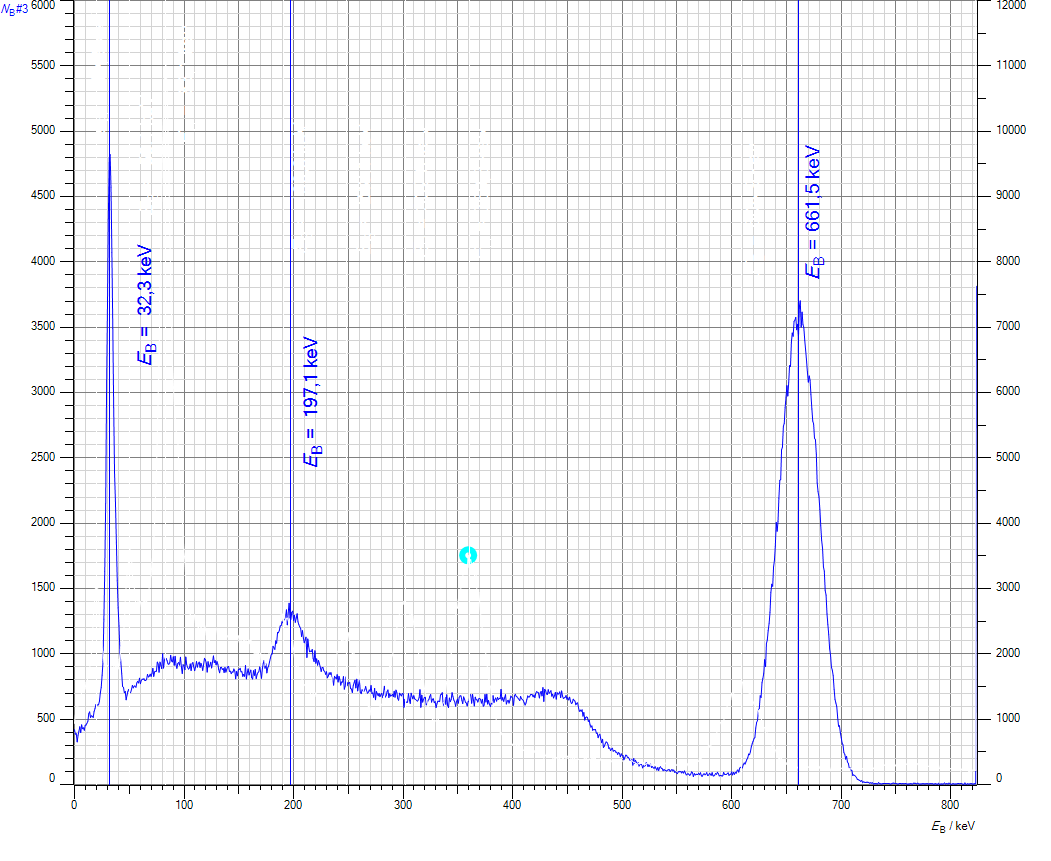
\includegraphics[width=0.95\textwidth]{./figures/c137kalibrierung.png}
  \end{center}
  \caption[Kalibrierungsmessung]{}
  \label{fig:kalibrierung}
\end{figure}



\subsection{Aufnahme des komplexen \texorpdfstring{$\gamma$}{gamma} Spektrums und seinen Zerfallsprodukten}

Der Versuch wird, wie zuvor beschrieben, wie in \autoref{aufbau_szinti}
aufgebaut, auch wird erneut eine Spannung von \SI{0.73}{\kilo\volt} verwendet.
Als radioaktive Quelle wird für diesen Teil des Versuchs das zu vermessende
\ch{^{226}_{88}Ra} verwendet. auch diese Werte werden auf den Computer
übertragen und den zuvor erzeugten Plot bei einer Laufzeit von
\SI{2400}{\second} beigefügt. Anhand des zuvor bestimmten Referenzspektums
können nun die Peaks des \ch{^{226}_{88}Ra} Spektrums vermessen werden.





\section{Auswertung}\label{sec:Auswertung}

\subsection{Messung der \texorpdfstring{$\alpha$}{alpha}, \texorpdfstring{$\beta$}{beta} und 
\texorpdfstring{$\gamma$}{gamma} Strahlung ohne und mit verschiedenen dicken Abschirmungen}



\subsection{Aufnahme der Zählrohrcharakteristik}




\subsection{Aufnahme der Zählstatistik}


\subsection{Bestätigung des Abstandsgesetzes}


\subsection{Bestimmung der Endpunktsenergie über Absorption in Aluminium}


\subsection{Aufnahme des Energiespektrums von \texorpdfstring{$\beta$}{beta} Strahlung mit Magnetspektrometer}


\subsection{Aufnahme und Kalibrierung des \texorpdfstring{$\gamma$}{gamma} Spektrums}


\subsection{Aufnahme des komplexen \texorpdfstring{$\gamma$}{gamma} Spektrums und seinen Zerfallsprodukten}






\section*{Diskussion}\label{sec:diskussion}


%verschieben der Hall sonde bei mag

\section{Zusammenfassung}



\newpage

\printbibliography
\listoffigures
\listoftables
\end{document}
